\documentclass{beamer}

\mode<presentation>
{
	\usetheme{CambridgeUS}
	\usecolortheme{orchid}
	\setbeamercovered{transparent}
	\useinnertheme{rectangles}
	\setbeamertemplate{navigation symbols}{}
	\usefonttheme[onlymath]{serif}
	\setbeamercolor{title}{bg=alerted text.fg!85!black, fg=white}
	\setbeamercolor{item projected}{bg=alerted text.fg!85!black}
	\setbeamertemplate{enumerate items}[default]
	\setbeamercolor{local structure}{fg=alerted text.fg!85!black}
}

\usepackage[english]{babel}
\usepackage[utf8]{inputenc}
\usepackage[T1]{fontenc}
\usepackage{lmodern}
\usepackage{pifont}
\usepackage{mathrsfs}
\usepackage{amsmath}
\usepackage{bm}
\usepackage{caption}
\usepackage{subcaption}
\usepackage{outlines}
\usepackage{multirow}
\usepackage{booktabs}
\usepackage[%
	autocite     = plain,
	doi          = true,
	url          = true,
	giveninits   = true,
	hyperref     = true,
	backref      = true,
	maxbibnames  = 99,
	maxcitenames = 99,
	sortcites    = true,
	style        = authoryear,
]{biblatex}

% \input{bibliography-mimosis}
\addbibresource{presentation.bib}

\newcommand{\fakeimage}{{\fboxsep=-\fboxrule\fbox{\rule{0pt}{3cm}\hspace{4cm}}}}

\usepackage{tikz}
\usetikzlibrary{shapes.symbols,shapes.geometric,shadows,arrows.meta}
\tikzset{
>={Latex[width=2mm,length=2mm]},
% Specifications for style of nodes:
base/.style = {shape=rectangle, rounded corners, draw=black, fill=blue!30,
                minimum width=1cm, minimum height=1cm, text centered},
multidocument/.style = {shape=tape, draw=black, fill=blue!30,
                minimum width=1cm, minimum height=1cm, text centered,
                tape bend top=none, double copy shadow},
database/.style = {shape=cylinder, draw=black, fill=blue!30, aspect=0.1,
                minimum height=2cm, minimum width=1cm, shape border rotate=90, text centered},
gene/.style = {shape=ellipse, draw=black, fill=blue!20, minimum width=1cm, minimum height=1cm, text centered},
mirna/.style = {shape=isosceles triangle, isosceles triangle apex angle=90, draw=black, fill=green!20, shape border rotate=90, minimum width=0.3cm, minimum height=0.1cm, text centered}
}


\definecolor{hdblue}{HTML}{3366cc}
\hypersetup{colorlinks,linkcolor=,urlcolor=hdblue, citecolor=hdblue}


\newcommand{\xmark}{\ding{55}}
\newcommand{\highlight}[1]{%
	\colorbox{red!50}{$\displaystyle#1$}}


\def\ci{\perp\!\!\!\perp}
\makeatletter
\newcommand*{\indep}{%
	\mathbin{%
		\mathpalette{\@indep}{}%
	}%
}
\newcommand*{\nindep}{%
	\mathbin{%                   % The final symbol is a binary math operator
		\mathpalette{\@indep}{\not}% \mathpalette helps for the adaptation
		% of the symbol to the different math styles.
	}%
}
\def\layersep{.38cm}
\def\inlsep{.4}
\newcommand*{\@indep}[2]{%
	% #1: math style
	% #2: empty or \not
	\sbox0{$#1\perp\m@th$}%        box 0 contains \perp symbol
	\sbox2{$#1=$}%                 box 2 for the height of =
	\sbox4{$#1\vcenter{}$}%        box 4 for the height of the math axis
	\rlap{\copy0}%                 first \perp
	\dimen@=\dimexpr\ht2-\ht4-.2pt\relax
	% The equals symbol is centered around the math axis.
	% The following equations are used to calculate the
	% right shift of the second \perp:
	% [1] ht(equals) - ht(math_axis) = line_width + 0.5 gap
	% [2] right_shift(second_perp) = line_width + gap
	% The line width is approximated by the default line width of 0.4pt
	\kern\dimen@
	{#2}%
	% {\not} in case of \nindep;
	% the braces convert the relational symbol \not to an ordinary
	% math object without additional horizontal spacing.
	\kern\dimen@
	\copy0 %                       second \perp
}
\makeatother


\title[Cancer Network]{Elucidation of MicroRNA-Gene Regulation in Human Cancer with Integrative Network Models}

% \subtitle
% {Presentation Subtitle} % (optional)

\author[Dogan]
{%
	\texorpdfstring{
		\begin{columns}
			\column{.85\linewidth}
			\centering
			Haluk Dogan, Zeynep Hakguder, Stephen Scott, and Juan Cui$^{*}$
		\end{columns}
	}
	{Dogan}
}
\institute[UNL] % (optional, but mostly needed)
{
  Systems Biology and Biomedical Informatics Laboratory\\
  \url{https://sbbi.unl.edu/}\\\vspace{1cm}
  Department of Computer Science and Engineering\\
  University of Nebraska-Lincoln
}

\date[\today] % (optional)
{\today}

\subject{Talks}

\pgfdeclareimage[height=0.5cm]{university-logo}{figures/logo}
\logo{\pgfuseimage{university-logo}}

% Delete this, if you do not want the table of contents to pop up at
% the beginning of each subsection:
\AtBeginSubsection[]
{
	\begin{frame}<beamer>{Outline}
		\tableofcontents[currentsection,currentsubsection]
	\end{frame}
}

%\tikzset{every picture/.style={line width=0.75pt}}

\begin{document}

\begin{frame}
  \titlepage{}
\end{frame}

\section{Introduction}
\begin{frame}{Introduction}
  Modeling interaction between cancer associated genes, miRNAs, and lncRNAs
  \begin{figure}[ht]
    \centering
    \includegraphics[width=0.8\textwidth, height=0.5\textheight]{figures/prob.jpeg}
    \caption*{\label{fig:prob} }
  \end{figure}
\end{frame}

\begin{frame}{Network Analysis}
	\begin{figure}[ht]
		\centering
		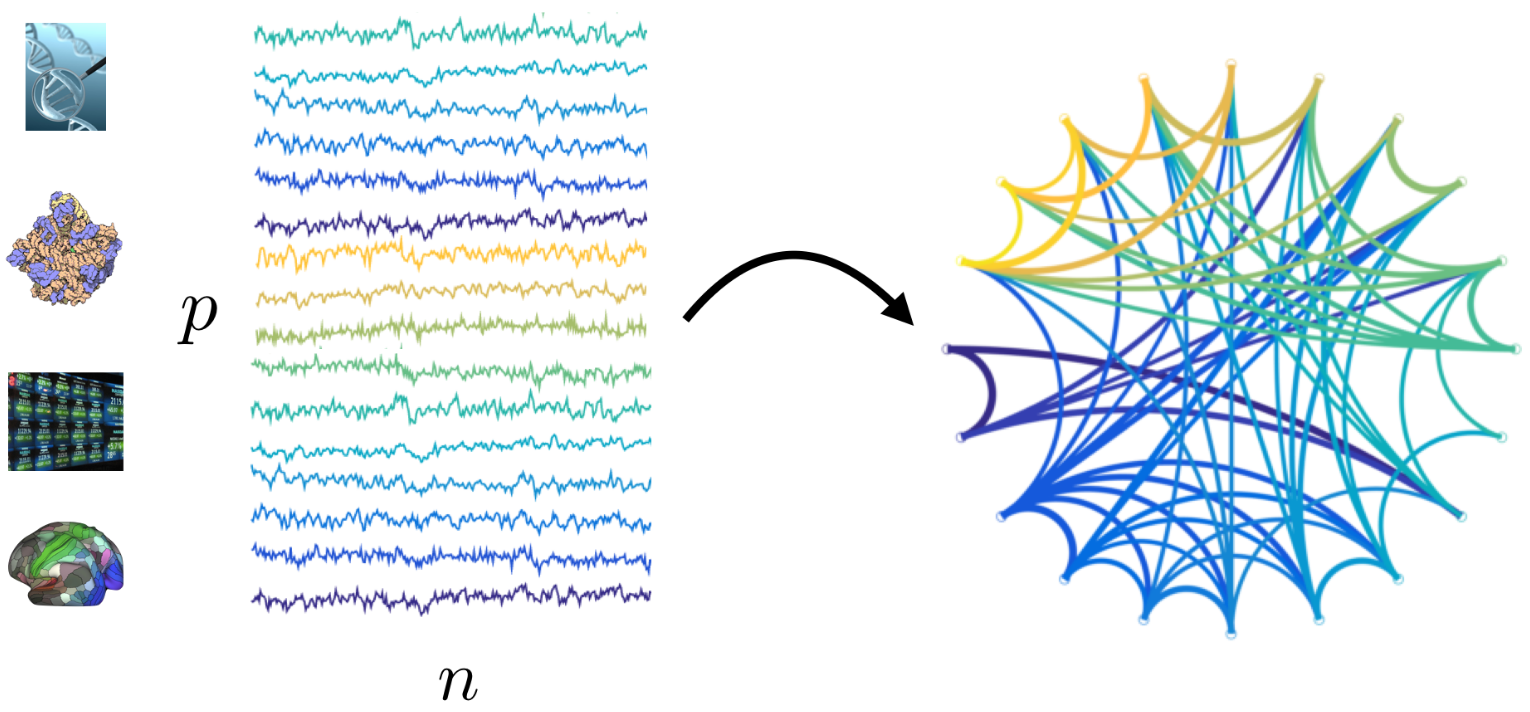
\includegraphics[width=1\textwidth]{figures/network.png}
		\caption*{\label{fig:network}}
	\end{figure}
\end{frame}
\begin{frame}{Network Analysis (cont'd)}
	\begin{columns}
		\begin{column}[t]{.48\textwidth}
			Correlation network:
			\begin{figure}[ht]
				\centering
				\includegraphics[width=0.5\textwidth]{figures/correlation.png}
				\caption*{\label{fig:correlation-network}}
			\end{figure}
			\vspace{-1.5cm}
			\begin{figure}[ht]
				\centering
				\includegraphics[width=1\textwidth,height=0.4\textheight]{figures/correlation-causation.png}
				\caption*{\label{fig:correlation-causation}}
			\end{figure}
		\end{column}
		\begin{column}[t]{.48\textwidth}
			Occam's razor:
			\begin{figure}[ht]
				\centering
				\includegraphics[width=1\textwidth,height=0.7\textheight]{figures/elephant.jpg}
				\caption*{\label{fig:elephant}}
			\end{figure}
		\end{column}
	\end{columns}
  \end{frame}
  \begin{frame}{Our Approach}
	\begin{figure}[ht]
	  \centering
	  \scalebox{0.7}{\input{figures/workflow.tikz}}
	\end{figure}

\end{frame}
\begin{frame}{Gaussian Graphical Models}
	Gene regulatory network:
	\begin{itemize}
		\item $\bm{X}=\left[X_{1}, X_{2}, \dots, X_{p}\right]$
		\item $\bm{X} \sim N(\bm{\mu}, \bm{\Sigma})$
		\item $P(\bm{X} ; \bm{\mu}, \bm{\Sigma})=\frac{1}{(2 \pi)^{p / 2}|\bm{\Sigma}|^{1 / 2}} \exp \left(-\frac{1}{2}(\bm{X}-\bm{\mu})^{T} \bm{\Sigma}^{-1}(\bm{X}-\bm{\mu})\right)$
		\item $\bm{\mu} \in \mathbb{R}^{p}, \boldsymbol{\Sigma} \in \mathbb{S}_{++}^{p}$
		\item Precision matrix: $\bm{\Theta} = \bm{\Sigma}^{-1}$
		\item Challenging problem when $n \ll p$\\
		      Assumptions:
		      \begin{itemize}
			      \item $\bm{\Theta}$ is sparse ($\ell_{1}$)
			      \item Models for each group should not be too different ($\ell_{2}$)
		      \end{itemize}
		\item $\text{Smoke} \ci \text{Heat} \mid \text{Fire}$
	\end{itemize}
\end{frame}
\begin{frame}{Gaussian Graphical Models (cont'd)}
  \begin{itemize}
	  \item $\mathcal{L}(\mathbf{\Omega}, \mathbf{x}) \equiv \log \operatorname{det}
	\boldsymbol{\Omega}-(\mathbf{x}-\boldsymbol{\mu})^{\top}
	\boldsymbol{\Omega}(\mathbf{x}-\boldsymbol{\mu})$
	  \item $\begin{aligned}[t] \mathcal{L}(\mathbf{\Omega},
		\mathbf{\widehat{\Sigma}}) & \equiv \frac{1}{N} \sum_{n}
		\mathcal{L}\left(\mathbf{\Omega}, \mathrm{x}^{(n)}\right) \\ &=\log
		\operatorname{det}
		\mathbf{\Omega}-\text{tr}(\widehat{\mathbf{\Sigma}}\mathbf{\Omega}) \end{aligned}$
	  \item $\min _{\{\mathbf{\Omega}>0\}} \mathcal{L}(\{\mathbf{\Omega}\})
		:= \sum _{ k=1  }^{ K }{ \text{tr}(\mathbf{\widehat{\Sigma}}^{(k)}\mathbf{\Omega}^{(k)})-\log
		\operatorname{det} \mathbf{\Omega}^{(k)}+P(\{\mathbf{\Omega}\})  }$
  \end{itemize}

\end{frame}
\begin{frame}{Data Augmentation}
	\begin{columns}
		\begin{column}{.48\textwidth}
			Conducting experiments:
			\begin{itemize}
				\item Unethical
				\item Expensive
				\item Difficult to repeat
			\end{itemize}
			\vspace{1cm}
			We used deep learning to generate more in-vitro samples:
			\begin{itemize}
				\item number of samples in groups is imbalanced
				\item unbiased estimator for a learner
			\end{itemize}
		\end{column}
		\begin{column}{.48\textwidth}
			\begin{figure}[ht]
				\centering
				\includegraphics[width=1\textwidth,height=0.7\textheight]{figures/deep-learning-image.jpg}
				\caption*{\label{fig:deep-learning}}
			\end{figure}
		\end{column}
	\end{columns}
\end{frame}
\begin{frame}{Constructing Bayesian Network}
  MiRNA Co-Binding Network:
	\begin{columns}
		\begin{column}[t]{.48\textwidth}
			\begin{figure}[ht]
				\centering
				\includegraphics[width=1\textwidth,height=0.3\textheight]{figures/mirna-cobinding.jpg}
				\caption*{\label{fig:mirna-cobinding}}
			\end{figure}
			\vspace{-1.5cm}
			\begin{figure}[ht]
				\centering
				\includegraphics[width=1\textwidth]{figures/directed.png}
				\caption*{\label{fig:directed}}
			\end{figure}
		\end{column}

		\begin{column}[t]{.48\textwidth}
			\begin{itemize}
				\item We constructed a Bayesian network to represent miRNA co-binding relationships
				\item Evidence matrix is from starBase
				      \begin{table}[]
					      \scalebox{0.7}{
						      \begin{tabular}{|c|l|l|l|l|}
							      \hline
							                  & Gene$_{1}$                                       & Gene$_{2}$ & $\dots$ & Gene$_{n}$ \\ \hline
							      miRNA$_{1}$ & \multicolumn{4}{c|}{\multirow{4}{*}{\huge{1/0}}}                                     \\ \cline{1-1}
							      miRNA$_{2}$ & \multicolumn{4}{l|}{}                                                                \\ \cline{1-1}
							      $\vdots$    & \multicolumn{4}{l|}{}                                                                \\ \cline{1-1}
							      miRNA$_{p}$ & \multicolumn{4}{l|}{}                                                                \\ \hline
						      \end{tabular}
						      \label{table:evidence-matrix}
					      }
				      \end{table}
				\item Intervention to a model is a lot easier
			\end{itemize}
		\end{column}
	\end{columns}
\end{frame}
\begin{frame}{Connecting Models}
	\begin{itemize}
		\item We test each miRNA and its dependencies to see if they make significant group difference
		\item We used a probabilistic distance metric to measure the data similarity with and without testing miRNAs and their dependencies
		      \begin{itemize}
			      \item Entropic Gromov Wasserstein
		      \end{itemize}
	\end{itemize}
	\begin{columns}
		\begin{column}{.48\textwidth}
			\begin{figure}[ht]
				\centering
				\includegraphics[width=0.7\textheight]{figures/earth-mover-distance.jpeg}
				\caption*{\label{fig:emd}}
			\end{figure}
		\end{column}
		\begin{column}{.48\textwidth}
			\begin{figure}[ht]
				\centering
				\scalebox{0.7}{\input{figures/connect-networks.tikz}}
				\caption*{\label{fig:connect-networks}}
			\end{figure}
		\end{column}
	\end{columns}
\end{frame}

\section{Results}
\begin{frame}{Data}
	\begin{columns}
		\begin{column}{.48\textwidth}
			\begin{itemize}
				\item Data: TCGA-BRCA
				\item Samples:
				      \begin{itemize}
					      \item Normal: 104
					      \item Stage 1: 179
					      \item Stage 2: 608
					      \item Stage 3: 242
					      \item Stage 4: 20
				      \end{itemize}
				\item DEGs (fold-change $> 2$):
				      \begin{itemize}
					      \item Up: 1218
					      \item Down: 1236
				      \end{itemize}
				\item 617 miRNAs
				      \begin{itemize}
					      \item 1,678 co-binding relationships
					      \item 20,441/166,669 bindings make significant group difference
				      \end{itemize}
			\end{itemize}
		\end{column}

		\begin{column}{.48\textwidth}
			\begin{figure}[ht]
				\centering
				\includegraphics[width=1\textwidth, height=0.7\textheight]{figures/diff-genes-volcano.png}
				\caption*{\label{fig:volcano}}
			\end{figure}
		\end{column}
	\end{columns}
\end{frame}

\begin{frame}{Results (cont'd)}
	\begin{columns}
		\begin{column}{.48\textwidth}
			\begin{figure}[ht]
				\centering
				\includegraphics[width=1\textwidth]{figures/original-data-heatmap.png}
				\caption*{\label{fig:original-heatmap}}
			\end{figure}
		\end{column}
		\begin{column}{.48\textwidth}
			\begin{figure}[ht]
				\centering
				\includegraphics[width=1\textwidth]{figures/data-aug.png}
				\caption*{\label{fig:data-aug}}
			\end{figure}
		\end{column}
	\end{columns}
\end{frame}
\begin{frame}{Results (cont'd)}
	\begin{figure}[ht]
		\centering
		\includegraphics[width=0.7\textwidth,keepaspectratio]{figures/network-venn.png}
		\caption*{\label{fig:network-venn}}
	\end{figure}
\end{frame}
\begin{frame}{Results (cont'd)}
	Disease Enrichment on lncRNAs:
	\begin{itemize}
		\item DOID:2449 acromegaly and \textbf{GATA3-AS1}
		\item DOID:299 adenocarcinoma and \textbf{PVT1}
		\item DOID:3355 fibrosarcoma, DOID:8791 breast carcinoma in situ, DOID:8719 in situ carcinoma and \textbf{LINC00987}
	\end{itemize}
\end{frame}
\begin{frame}{Results (cont'd)}
	Low degree miRNAs that make group difference:
	\begin{columns}
		\begin{column}[t]{.48\textwidth}
			\begin{itemize}
				\item hsa-miR-129-5p
				\item hsa-miR-140-3p
				\item hsa-miR-146b-5p
				\item hsa-miR-188-5p
				\item hsa-miR-193a-5p
				\item hsa-miR-28
				\item hsa-miR-346
				\item hsa-miR-3605-3p
			\end{itemize}
		\end{column}
		\begin{column}[t]{.48\textwidth}
			\begin{itemize}
				\item hsa-miR-361
				\item hsa-miR-455-5p
				\item hsa-miR-671-3p
				\item hsa-miR-320b
				\item hsa-miR-193a-3p
				\item hsa-miR-326
				\item hsa-miR-330
				\item hsa-miR-501-3p
			\end{itemize}
		\end{column}
	\end{columns}
  \end{frame}

  \begin{frame}{Acknowledgement}
	\begin{figure}[ht]
	  \centering
	  \includegraphics[height=0.6\textheight,keepaspectratio]{figures/sbbi.jpg}
	  \caption*{\label{fig:sbbi}}
	\end{figure}
	\vspace{-1cm}
	\begin{figure}[ht]
	  \centering
	  \includegraphics[height=0.2\textheight,keepaspectratio]{figures/hcc.png}
	  \caption*{\label{fig:hcc}}
	\end{figure}

	\end{frame}

\section{Conclusion}
\begin{frame}{Questions}
	\begin{center}
		\Huge{Questions?}
	\end{center}
	\begin{figure}
		\centering
		\includegraphics[width=0.5\textwidth, height=1.0\textheight, keepaspectratio]{figures/walter.jpg}
	\end{figure}
\end{frame}
% \begin{frame}[allowframebreaks]
% 	\frametitle{References}
% 	% \bibliographystyle{chicago}
% 	% \bibliography{presentation}
% 	\printbibliography{}
% \end{frame}
\end{document}

%%% Local Variables:
%%% mode: latex
%%% TeX-master: t
%%% End:
